\documentclass[journal,a4paper]{IEEEtran}
% Two-column IEEE journal format (IEEEtran is built into Overleaf). Compile with pdfLaTeX.
\usepackage[T1]{fontenc}
\usepackage{cite}
\usepackage{amsmath,amssymb}
\usepackage{graphicx}
\usepackage{booktabs}
\usepackage{tabularx}
\usepackage{array}
\usepackage{xcolor}
\usepackage{enumitem}
\usepackage{url}
\usepackage[hidelinks]{hyperref}
\setlist{nosep,leftmargin=1.4em}
\newcolumntype{L}{>{\raggedright\arraybackslash}X}
% shrink a table to the line width only if it is wider (never enlarge it)
\newcommand{\fitwidth}[1]{\resizebox{\ifdim\width>\linewidth\linewidth\else\width\fi}{!}{#1}}
% many full-width figures/tables: relax float placement so that they stay near their text
\extrafloats{100}
\renewcommand{\topfraction}{0.9}\renewcommand{\bottomfraction}{0.8}
\renewcommand{\textfraction}{0.07}\renewcommand{\floatpagefraction}{0.75}
\renewcommand{\dbltopfraction}{0.9}\renewcommand{\dblfloatpagefraction}{0.75}
\setcounter{topnumber}{3}\setcounter{dbltopnumber}{3}\setcounter{totalnumber}{6}
\graphicspath{{C4_images/}}
\setlength{\emergencystretch}{1.5em} % fewer overfull lines in the narrow columns
% Instructor's convention: a value that is NOT a real measured result is written as \nr{95.7},
% which prints [95.7] in red. Real results are printed normally (black).
% Every number in this draft is a real result from the repository's results/ folder,
% so \nr is not used anywhere in this version.
\newcommand{\nr}[1]{\textcolor{red}{[#1]}}

\begin{document}
\title{Does the Forecaster Matter? A Causal, Budget-Constrained Evaluation of Prophet--LSTM Predictive
Autoscaling in Kubernetes}
\author{Saad Azhar (i230822) and Syed Ali Ramish Abidi (i230651)%
\thanks{S.~Azhar and S.~A.~R.~Abidi are with the Department of Computer Science, FAST-NUCES Islamabad,
Pakistan (e-mail: i230822@isb.nu.edu.pk; i230651@isb.nu.edu.pk). Cloud Computing Research, Group~35.
Supervisor: Basharat Hussain.}}
\markboth{Cloud Computing Research, Group 35, FAST-NUCES Islamabad --- Day-80 Complete Draft, November 2026}{Azhar and Abidi: Causal, Budget-Constrained Evaluation of Prophet--LSTM Autoscaling}
\maketitle

\begin{abstract}
Predictive autoscalers forecast the request rate of a service and provision pods before demand arrives.
Hybrid forecasters such as Prophet--LSTM report large accuracy gains over single models, but they are evaluated
offline and never measured inside the controller that must run them. We ask whether a Prophet--LSTM forecaster
can run within a Kubernetes controller's CPU budget, produce timely and causally valid forecasts, and improve
scaling decisions over the reactive Horizontal Pod Autoscaler (HPA) and over lightweight forecasters. We built a
budget-aware KEDA external scaler that runs the forecaster under a CPU limit (100m--500m) and a deadline with a
persistence fallback, a trace-driven simulator, and a live kind/Prometheus testbed, and we evaluated them on the
NASA-HTTP and WorldCup98 traces with one replica policy shared by every autoscaler.
First, the published evaluation is non-causal: corrected, the hybrid's RMSE is 43\,\% (NASA) and 40\,\% (FIFA)
higher, and AR(10) is more accurate on both traces. Second, per-decision inference fits every budget down to 25m (266\,ms CPU
and 2.9\,s p95 latency at 100m), but forecasts become late for deadlines of 2\,s or less at 100m, and the binding
costs are cold start (270\,s at 100m, 14\,min at 25m), about 0.7\,GB of memory and re-fitting, which cannot share
the budget.
Third, request-rate scaling reduces under-provisioning compared with the CPU-based HPA (live, three seeds: $\Theta_U$
21.1\,\%$\to$0.9\,\% at 100m), but a persistence forecaster obtains the same gain (live: 0.8\,\%; simulated:
statistically indistinguishable on ramping and bursty load), and Prophet alone fails on flash crowds. The benefit therefore comes from the scaling signal, not from
the forecaster.
All code, trained models, raw results and scripts needed to reproduce every result in this paper are publicly available at \url{https://github.com/Saadx-git/Cloud_project_I230822_I230651}.
\end{abstract}

\begin{IEEEkeywords}
Kubernetes, predictive autoscaling, time-series forecasting, Prophet--LSTM, controller overhead, reproducibility.
\end{IEEEkeywords}

\section{Introduction}
\IEEEPARstart{E}{lasticity} is the defining operational property of cloud-native services. In Kubernetes, the Horizontal Pod
Autoscaler (HPA) adjusts the number of replicas of a workload from an observed metric, by default CPU
utilisation~\cite{burns2016,nguyen2020}.\footnote{Kubernetes documentation, ``Horizontal Pod Autoscaling'', \url{https://kubernetes.io/docs/concepts/workloads/autoscaling/horizontal-pod-autoscale/}.} The HPA is \emph{reactive}: it acts only after utilisation has crossed its
target, and the new pods need time to start. Under sudden load increases this produces a window of
under-provisioning and service-level objective (SLO) violations, and operators compensate with over-provisioning.

Predictive (proactive) autoscaling addresses this by forecasting demand one control period ahead and provisioning
for the forecast~\cite{lorido2014,qu2018,aldhuraibi2018,dogani2023}. A large body of work proposes ever more sophisticated forecasters for
this purpose, from ARIMA~\cite{calheiros2015} to LSTM and Bi-LSTM networks~\cite{imdoukh2020,dangquang2021} and
hybrid models. A recent example, published in \emph{Frontiers in Computer Science}, is the Prophet--LSTM hybrid of
Guruge and Priyadarshana~\cite{guruge2025}. Prophet~\cite{taylor2018} models trend and seasonality, an
LSTM~\cite{hochreiter1997} models Prophet's residual, and the authors report a 65--90\,\% accuracy improvement
over single models on the NASA-HTTP and WorldCup98 traces.

Two questions are left open by such work. The first is whether the accuracy gain is real. In our reproduction of
the base paper (Cutoff~2) we found that its evaluation scores the forecast for minute $t{+}1$ against minute $t$,
so the reported forecast contains the value it predicts. The second is whether the forecaster can run where it
would actually be deployed: inside an autoscaling controller that is itself a Pod with a CPU limit, that must
return a decision every control period, and that must start, restart and re-train within that budget. Neither
the base paper nor, to our knowledge, the related work measures the forecaster inside such a budget.

This paper studies both questions end to end. Our contributions are:
\begin{enumerate}[label=C\arabic*]
\item A \textbf{causal re-evaluation} of the Prophet--LSTM autoscaler that quantifies how much the non-causal
      protocol inflates both forecast accuracy and downstream scaling quality, against six reference forecasters.
\item A \textbf{budget-aware KEDA external scaler} that runs any forecaster under a CPU limit and a decision
      deadline with a persistence fallback, together with a measurement of its cost (CPU per decision, latency,
      deadline misses, cold start, memory, re-fitting) as a function of the CPU budget.
\item A \textbf{controlled comparison} of reactive and predictive autoscalers that share one replica policy, so
      that differences are caused only by the scaling signal, in a trace-driven simulator (four scenarios) and on a
      live Kubernetes cluster with repeated runs and block-bootstrap confidence intervals.
\item A \textbf{public reproducibility package} with code, trained models, raw results and figure scripts.
\end{enumerate}


%=====================================================================
\section{Problem and Motivation}\label{sec:problem}
\paragraph{Problem.} A predictive autoscaler is a control loop. Every control period $P$ it observes the request
rate $y_t$, forecasts $\hat y_{t+1}$, converts the forecast into a replica count and actuates it. The value of a
forecaster to this loop depends on three properties that offline accuracy tables do not capture:
\begin{enumerate}
\item \textbf{Causality.} The forecast for $t{+}1$ may only use information available at $t$. An evaluation that
      violates this measures something other than forecasting skill.
\item \textbf{Timeliness under a budget.} The forecast must be ready before the decision is due, on the CPU that
      the controller is allowed to use. In Kubernetes this budget is the controller Pod's CPU limit, enforced by
      the Linux CFS quota. A model that is fast on an unconstrained workstation can be slow when throttled to
      a tenth of a core.
\item \textbf{Decision value.} What matters is the quality of the resulting replica counts (under- and
      over-provisioning, SLO violations, pod-minutes), not the forecast error itself, and it must be compared
      with the cheapest alternative signals.
\end{enumerate}

\paragraph{Motivation.} Controllers are given small, fixed resources, because they run on every cluster and
their cost is pure overhead. A hybrid deep-learning forecaster brings a large runtime (TensorFlow, Stan), hundreds
of megabytes of memory and periodic re-training. If its gain over a last-value forecaster is small, or exists only
under a flawed evaluation, its cost is not justified; if the gain is real and fits a realistic budget,
practitioners obtain a concrete deployment envelope. Either answer requires measurement inside a real control loop.

%=====================================================================
\section{Research Questions and Objectives}\label{sec:rq}
\begin{quote}\itshape
Primary RQ: Can a Prophet--LSTM hybrid forecaster run within a Kubernetes controller's CPU budget, produce timely
and causally valid forecasts, and improve scaling decisions compared with the reactive HPA and with lightweight
forecasters?
\end{quote}
We decompose it into three sub-questions:
\begin{itemize}
\item \textbf{RQ1 (validity).} How much does the non-causal evaluation of the base paper inflate forecast accuracy
      and scaling quality, and how does the hybrid rank against simple forecasters under a causal protocol?
\item \textbf{RQ2 (cost and timeliness).} What does the hybrid cost inside a CPU-limited controller (CPU per
      decision, latency, cold start, memory, re-fitting), and at which budget and deadline do forecasts become
      late?
\item \textbf{RQ3 (benefit).} Under one shared replica policy, does the hybrid reduce under-provisioning and SLO
      violations compared with the HPA, and compared with a persistence forecaster, and at what resource cost?
\end{itemize}
The objectives are to (O1)~quantify $t{+}1$ forecast quality under a causal protocol and the inflation caused by
the leaky one (E1; RQ1); (O2)~measure the controller-side cost of each forecaster as a function of the CPU limit
and the deadline (E2, E5; RQ2); (O3)~compare HPA and predictive scalers under one replica policy on four
scenarios with bootstrap confidence intervals (E3, E5; RQ1, RQ3); and (O4)~validate the comparison on a live
Kubernetes cluster with repeated runs (E4; RQ2, RQ3).

%=====================================================================
\section{Literature Review}\label{sec:lit}
We organise the literature into four themes: the reactive baseline and production practice, forecasting-based
autoscaling, hybrid and ensemble forecasters, and evaluation methodology. Table~\ref{tab:lit} compares the most
relevant studies.

\subsection{Reactive autoscaling and production practice}
Surveys classify autoscalers into threshold rules, control theory, queueing models, reinforcement learning and
time-series forecasting~\cite{lorido2014,qu2018,aldhuraibi2018}. More recent surveys cover container-based and
edge platforms~\cite{dogani2023}, reinforcement-learning autoscalers~\cite{gari2021} and machine-learning-based
container orchestration~\cite{zhong2022}. Threshold rules dominate in practice because they are simple and
predictable. The Kubernetes HPA is such a rule: it scales the replica count in proportion to the ratio between
the observed and the target metric, ignores changes within a 10\,\% tolerance and delays scale-down by a
stabilisation window, as specified in the Kubernetes documentation. Nguyen et al.~\cite{nguyen2020} show experimentally that the HPA's behaviour
depends strongly on the metric source and on the scraping and synchronisation periods. They also show that custom
metrics from Prometheus can make it react more accurately than the default resource metrics. Burns et
al.~\cite{burns2016} describe how Kubernetes inherited from Google's Borg and Omega the design of simple controllers,
each of which repeatedly reconciles an observed state with a desired one. Gandhi et al.~\cite{gandhi2012} show for
multi-tier data centres that a policy which does not predict load, but accounts for server set-up time and
releases capacity conservatively, handles unpredictable load robustly and compares favourably with
prediction-based policies. \emph{Synthesis:} production systems
favour simple, cheap signals. The research literature rarely asks whether its more complex forecasters satisfy
the operational constraints that drive this preference.

\subsection{Forecasting-based (proactive) autoscaling}
Calheiros et al.~\cite{calheiros2015} used ARIMA to forecast web request rates and showed in simulation that
accurate forecasts improve QoS and utilisation. Kumar and Singh~\cite{kumar2018} trained a neural network with
adaptive differential evolution on web-server traces and reported lower error than gradient-trained networks.
For containers, Imdoukh et al.~\cite{imdoukh2020} proposed an LSTM-based autoscaler evaluated on the WorldCup98
trace and compared it with ARIMA. Dang-Quang and Yoo~\cite{dangquang2021} proposed a Bi-LSTM autoscaler for
Kubernetes evaluated on NASA-HTTP and WorldCup98, and introduced the under/over-provisioning metrics and the
scale-down ratio later reused by the base paper. Joshi et al.~\cite{joshi2024} combined ARIMA forecasts with a PID
controller to stabilise container scaling. Lanciano et al.~\cite{lanciano2024} extended OpenStack Monasca with
predictive elasticity and compared several forecasting models inside a real monitoring stack. Surveys of
workload prediction in clouds~\cite{amiri2017,masdari2020} catalogue dozens of such models but compare them mainly
by prediction error. Bauer et al.~\cite{bauer2020} review forecasting for self-aware systems and conclude that no
single method performs best on all time series, which motivates automatic method selection. \emph{Synthesis:}
these works share three assumptions. Forecast accuracy is used as the main proxy for scaling quality; the
forecaster is assumed to run on adequate resources; and the reactive baseline is CPU-based. The forecast is
rarely compared with a last-value signal fed into the same replica policy, so the effect of \emph{forecasting}
is not separated from the effect of the \emph{metric} that is scaled on.

\subsection{Hybrid and ensemble forecasters}
Hybrids aim to combine the strengths of statistical and learned models. Guruge and
Priyadarshana~\cite{guruge2025} decompose the series with Prophet and model the residual with a two-layer LSTM.
They report MSE improvements of 65--90\,\% over ARIMA, LSTM and Bi-LSTM on NASA-HTTP and WorldCup98, and list
prediction time and Kubernetes integration as future work. Chameleon~\cite{bauer2019} combines several
proactive methods with a reactive fallback and is benchmarked against reactive and proactive autoscalers on a
``level playing field''. Toka et al.~\cite{toka2021} run several forecasters (including AR and LSTM) in parallel
and select the currently best one online for Kubernetes edge clusters, with a single parameter trading
over-provisioning against SLA violations. Outside autoscaling, the M4 competition~\cite{makridakis2020} was won
by a hybrid of exponential smoothing and a recurrent network, while pure machine-learning methods performed poorly,
and Hewamalage et al.~\cite{hewamalage2021} find that recurrent networks can match statistical benchmarks, but
only with careful preprocessing and tuning. \emph{Synthesis:} hybrids and ensembles increase accuracy and
robustness at the price of more computation. Chameleon and Toka et al.\ motivate fallbacks and model selection,
but they do not quantify the controller's own CPU and memory budget as a constraint.

\subsection{Evaluation methodology}
Herbst et al.~\cite{herbst2018} define elasticity metrics (accuracy of under- and over-provisioning, and the share
of time in each state) that allow autoscalers to be compared independently of the forecaster. The base paper's
$\Theta_U,\Theta_O,T_U,T_O$ are of this kind. In forecasting research, the M-competition analysis of Makridakis et
al.~\cite{makridakis2018} found that simple statistical methods often match or beat machine-learning methods at
much lower computational cost, which makes simple baselines mandatory. Kapoor and Narayanan~\cite{kapoor2023}
document data leakage as a widespread cause of irreproducible machine-learning results, including the use of
information unavailable at prediction time. When leakage is corrected, complex models often lose their advantage
over simple ones. Tashman~\cite{tashman2000} reviews out-of-sample evaluation of forecasts, and Bergmeir and
Ben\'itez~\cite{bergmeir2012} compare cross-validation and out-of-sample schemes for time-series predictors; both
require a strict separation between the information used to produce a forecast and the data it is scored on.
Hyndman and Koehler~\cite{hyndman2006} recommend scaling errors relative to a naive (persistence) forecast, and
Diebold and Mariano~\cite{diebold1995} provide a test of whether two forecasters differ significantly in accuracy. Both traces used here are well characterised~\cite{arlitt1997,arlitt2000}: NASA-HTTP shows strong
daily and weekly cycles, and WorldCup98 shows extreme, match-driven flash crowds. \emph{Synthesis:} the field has
the metrics and the methodological warnings needed for a sound evaluation. They have not yet been applied
together to a forecaster running inside a constrained Kubernetes controller.

\begin{table*}[!t]\centering
\caption{Comparison of the most relevant studies (problem, method, setup, metrics, findings and remaining gap).}\label{tab:lit}
\scriptsize
\begin{tabularx}{\textwidth}{@{}>{\raggedright\arraybackslash}p{1.75cm}LLLLLL@{}}\toprule
Study & Problem & Method & Dataset / setup & Metrics & Finding & Gap w.r.t.\ this work \\ \midrule
Calheiros et al.\ 2015~\cite{calheiros2015} & Proactive VM provisioning & ARIMA & Wikimedia requests; CloudSim & Forecast error, QoS & Forecasts improve QoS & No controller cost; no causal/naive comparison of decisions \\
Imdoukh et al.\ 2020~\cite{imdoukh2020} & Container autoscaling & LSTM vs.\ ARIMA & WorldCup98 & Accuracy, prediction time & LSTM competitive with ARIMA & Offline timing; no CPU budget \\
Dang-Quang \& Yoo 2021~\cite{dangquang2021} & K8s autoscaling & Bi-LSTM & NASA, WorldCup98 & RMSE, $\Theta_U$, $\Theta_O$ & Bi-LSTM beats ARIMA & No live budgeted controller; no persistence baseline \\
Nguyen et al.\ 2020~\cite{nguyen2020} & HPA behaviour & Experiments on HPA & K8s cluster & Response time, replicas & Metric source and periods matter & Reactive only \\
Toka et al.\ 2021~\cite{toka2021} & Edge K8s scaling & Online selection of AR/HTM/LSTM & Web traces; K8s & SLA violations, resources & Selection beats single models & Controller overhead not budgeted \\
Bauer et al.\ 2019~\cite{bauer2019} & Robust proactive scaling & Hybrid ensemble + reactive fallback & Private/public clouds & SPEC elasticity metrics & Hybrid most robust & No CPU-limited controller \\
Gandhi et al.\ 2012~\cite{gandhi2012} & Data-centre capacity management & Non-predictive, set-up-aware scaling & Multi-tier server testbed & Response time, servers & Conservative non-predictive policy is robust & Not containers; no forecaster cost \\
Joshi et al.\ 2024~\cite{joshi2024} & Stable scaling & ARIMA + PID & Containers & Response time, replicas & PID smooths decisions & Forecast cost unmeasured \\
Lanciano et al.\ 2024~\cite{lanciano2024} & Predictive elasticity & Several forecasters in Monasca & OpenStack & Accuracy, scaling & Predictors integrated in monitoring & Not K8s; budget not varied \\
Guruge \& Priyadarshana 2025~\cite{guruge2025} & K8s request forecasting & Prophet--LSTM hybrid & NASA, WorldCup98 & MSE, RMSE, $R^2$, TPT & 65--90\,\% better than single models & Leaky evaluation; no live controller; batch timing only \\
\bottomrule\end{tabularx}
\end{table*}

%=====================================================================
\section{Research Gap}\label{sec:gap}
The literature supports three observations. (i)~Forecasting-based autoscalers are evaluated mainly by offline
accuracy, and the leading hybrid's accuracy advantage depends on a non-causal evaluation (our Cutoff~2
reproduction, confirmed in E1). (ii)~Prediction time is reported, if at all, as batch throughput on unspecified
hardware. No study we found measures the forecaster inside a CPU-limited controller, where throttling, cold start,
memory and re-training compete for the same small budget. (iii)~Predictive scalers are compared with a CPU-based
HPA, so a better result may come from scaling on the request rate rather than from forecasting. A persistence
forecaster in the same replica policy is the control that separates the two effects, and it is rarely
included~\cite{makridakis2018,kapoor2023,hyndman2006}.

\textbf{Gap.} \emph{There is no causal, end-to-end evaluation of a hybrid deep forecaster running inside a
CPU-budgeted Kubernetes controller that separates the value of forecasting from the value of the scaling signal.}
Our research question addresses exactly this combination. The gap is defensible because the base paper names
prediction time and Kubernetes integration as open problems, and the related work covers forecaster comparison
(Toka, Lanciano) or controller robustness (Chameleon) but not the interaction between the controller's budget,
the forecaster's complexity and a shared scaling policy.

%=====================================================================
\section{Methodology}\label{sec:method}
\subsection{Research design}
The study is experimental and comparative. Factors are the forecaster (seven levels), the CPU budget of the
controller (25m--1000m and unlimited), the decision deadline, the workload scenario (four) and the evaluation
protocol (causal vs.\ leaky). The design isolates the effect of each factor. All autoscalers share one replica
policy, so that differences in scaling quality are caused only by the input signal. Offline experiments (E1, E3)
cover the full factor space cheaply, and live experiments (E2, E4) measure what simulation cannot: throttling,
cold start, memory and real pod dynamics. E5 adds the statistical analysis.

\subsection{System under test}
Figure~\ref{fig:arch} shows the framework. It has four components.
\begin{itemize}
\item \textbf{Workload service.} A CPU-bound HTTP service in which every request performs a fixed PBKDF2
      computation. CPU use is therefore proportional to the request rate, and a pod has a well-defined capacity
      $C$ (requests/s at 100\,\% of its CPU request).
\item \textbf{Load generator.} It replays a trace slice open-loop with Poisson arrivals at rate
      $\lambda=y_{\text{trace}}\cdot s$. One trace minute is replayed in 15\,s of wall time.
\item \textbf{Monitoring.} Prometheus scrapes the service every 5\,s; metrics-server provides CPU at 15\,s
      resolution for the HPA.
\item \textbf{Budgeted predictive scaler.} A KEDA external scaler\footnote{KEDA documentation, ``External scalers'', \url{https://keda.sh/docs/2.16/concepts/external-scalers/}.} (gRPC). Every control period $P$ it reads the
      request rate of the last period from Prometheus and sends a forecast request to a worker process that holds
      the model. It waits at most $D$ seconds and publishes the forecast, which KEDA's HPA converts into replicas.
      If the deadline is missed, the persistence value $y_t$ is published, and the worker is killed and
      re-spawned. The gRPC \texttt{GetMetrics} call only returns the latest published value, so KEDA's own
      timeouts never interact with inference time. The scaler's CPU budget is the CFS quota of its Pod
      (\texttt{resources.limits.cpu}), the same mechanism that Kubernetes applies to every controller.
\end{itemize}

\begin{figure*}[!t]\centering
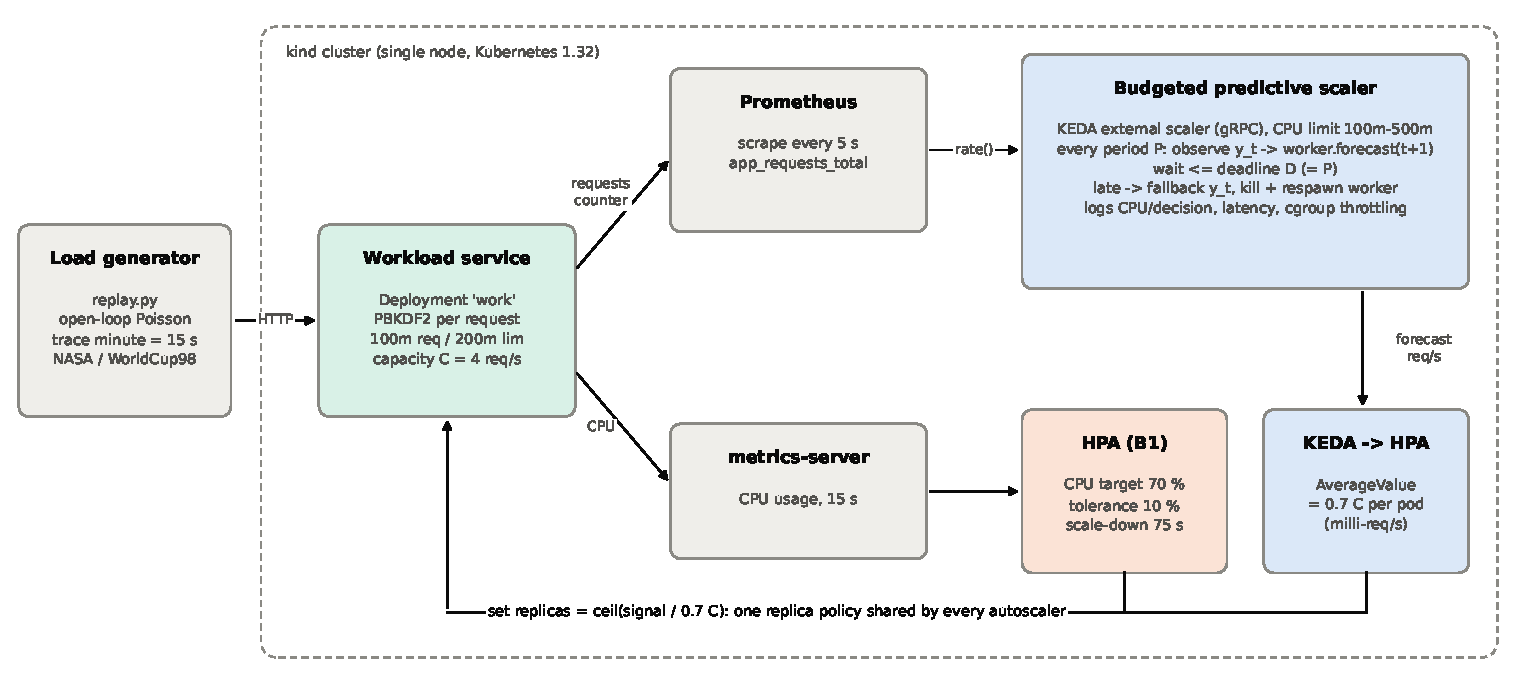
\includegraphics[width=0.82\textwidth]{fig_architecture.pdf}
\caption{Experimental framework (live setting, E4). E2 runs the same scaler image under \texttt{docker --cpus};
E3 replaces the cluster with a trace-driven simulator that implements the same replica policy.}\label{fig:arch}
\end{figure*}

\subsection{Compared autoscalers and the shared replica policy}
Every autoscaler uses the rule
\[
  N_{t+1}=\Big\lceil \frac{\text{signal}}{0.7\,C} \Big\rceil,
\]
with the HPA's 10\,\% tolerance, immediate scale-up and a scale-down stabilisation window of 5 control periods
(300\,s at a 60\,s step; 75\,s in the time-compressed live runs).
\begin{itemize}
\item \textbf{B1 -- HPA (reactive).} The signal is the observed CPU utilisation in period $t$. It saturates at the
      pod CPU limit (200\,\% of the request), as in a real cluster.
\item \textbf{B2 -- Prophet scaler.} The signal is Prophet's $\hat y_{t+1}$ with the released hyperparameters
      (changepoint prior 5.1, seasonality prior 30, weekly/daily Fourier orders 20/50, linear growth for NASA and
      flat growth for FIFA).
\item \textbf{Budgeted Prophet--LSTM (studied).} $\hat y_{t+1}=\hat y^{P}_{t+1}+\mathrm{LSTM}(y_t-\hat y^{P}_t)$
      with the released architecture (2$\times$50 LSTM, look-back 1), under a CPU limit of 100m--500m and a
      deadline $D$. Each model is run \emph{as released} (Prophet with 1000 uncertainty samples and
      \texttt{keras.Model.predict}) and \emph{optimised} (no uncertainty sampling and a direct model call; the
      point forecasts are identical).
\item \textbf{Lightweight references.} Persistence ($\hat y_{t+1}=y_t$), 5-minute moving average, seasonal naive
      (1 day) and AR(10) fitted by least squares on the training split.
\item \textbf{Oracle} (simulation only). The true $y_{t+1}$; it gives the best achievable result of the policy.
\end{itemize}

\subsection{Causal evaluation protocol}
Models are trained on the chronological first 70\,\% of each trace and evaluated on the remaining 30\,\%, as in
the base paper. Two corrections are applied, and the original variant is kept as a labelled \emph{leaky}
condition:
\begin{itemize}
\item \textbf{Alignment (fixes finding F1 of Cutoff~2).} A forecast is written to the row it forecasts, and its
      inputs are limited to rows before it.
\item \textbf{Scaler fitting (fixes F2).} The residual Min--Max scaler is fitted on training residuals only.
\end{itemize}
In the live scaler, Prophet is queried at the \emph{trace} timestamp of the replayed minute. This avoids the
30-year extrapolation of the released KEDA scaler (F4). We also corrected three defects that we found in the
released scaler: a unit mismatch between req/s and req/min (F7), a residual computed against the forecast for
$t{+}1$ instead of $t$ (F8), and truncation of the pod count (F9).

\subsection{Workloads}
Both traces are the per-minute request counts released with the base paper: NASA-HTTP (July--August
1995)~\cite{arlitt1997} and WorldCup98 (April--July 1998)~\cite{arlitt2000}. Four scenarios are cut from the test
splits (Table~\ref{tab:scen}), each preceded by 1500 minutes of history for forecaster warm-up. They cover low
noisy load (\texttt{steady}), a weekday cycle (\texttt{diurnal}), a gradual ramp (\texttt{ramp}, the slice used by
the base paper's autoscaler notebook) and a flash crowd (\texttt{bursty}, the semi-final of 7 July 1998).

\begin{table*}[!t]\centering
\caption{Workload scenarios (test split only). Length in minutes; mean and max in requests/minute; CV:
coefficient of variation; p99 step: 99th percentile of the absolute minute-to-minute relative change; ACF(1):
lag-1 autocorrelation.}\label{tab:scen}
\scriptsize
\fitwidth{\begin{tabular}{llllrrrrrrr}
\toprule
Scenario & Trace & Window & Type & Length (min) & Mean & Max & CV & Peak/mean & p99 step & ACF(1) \\
\midrule
steady & NASA & 1995-08-26 00:00 -- 00:00 & steady & 1440 & 22 & 87 & 0.59 & 3.96 & 650\% & 0.571 \\
ramp & FIFA & 1998-07-07 09:51 -- 16:32 & gradual ramp & 401 & 15,450 & 21,827 & 0.25 & 1.41 & 14\% & 0.981 \\
bursty & FIFA & 1998-07-07 18:00 -- 23:00 & bursty & 300 & 95,099 & 229,426 & 0.60 & 2.41 & 12\% & 0.998 \\
diurnal & NASA & 1995-08-22 00:00 -- 00:00 & diurnal & 1440 & 40 & 140 & 0.61 & 3.49 & 307\% & 0.744 \\
\bottomrule
\end{tabular}
}
\end{table*}

\subsection{Metrics}
\begin{itemize}
\item \textbf{Forecast quality} at $t{+}1$: RMSE, MAE and $R^2$ in raw requests/minute; RMSE is also reported
      relative to persistence, following~\cite{hyndman2006}.
\item \textbf{Controller cost}: CPU time per decision (\texttt{process\_time}, all threads), wall latency
      (p50/p95/max), cold start (import, model load and first call), resident memory, CFS throttling ratio, share
      of the period's CPU budget used, and the cost of re-fitting (Prophet on the last 7 days plus one LSTM
      epoch).
\item \textbf{Timeliness}: late-forecast fraction $\Pr[\text{latency}>D]$ for deadlines $D$ from 0.5\,s to the
      control period, and cold start expressed in control periods.
\item \textbf{Scaling quality}~\cite{herbst2018,dangquang2021}: with demand $r_t$ and provisioned capacity $p_t$
      (ready pods $\times\,0.7C$),
      \begin{align*}
      \Theta_U&=\tfrac{100}{T}\textstyle\sum_t \tfrac{\max(r_t-p_t,0)}{r_t}, &
      T_U&=\tfrac{100}{T}\#\{r_t>p_t\},\\
      \Theta_O&=\tfrac{100}{T}\textstyle\sum_t \tfrac{\max(p_t-r_t,0)}{r_t}, &
      T_O&=\tfrac{100}{T}\#\{p_t>r_t\},
      \end{align*}
      plus pod-minutes and, live, the share of requests violating a 500\,ms latency SLO (error, timeout or slower
      than 500\,ms).
\end{itemize}

\subsection{Statistical analysis}
Simulated scaling metrics are deterministic for a given trace, but they are averages over autocorrelated minutes.
We therefore compare two scalers by the paired difference of their per-minute contributions and estimate a 95\,\%
confidence interval with a moving-block bootstrap~\cite{kunsch1989}, an extension of the bootstrap~\cite{efron1979} to dependent data
(see also the stationary bootstrap~\cite{politis1994}) (block length 30 minutes, 2000 resamples).
A difference is called significant when the interval excludes zero. For the live experiment, each autoscaler is
repeated with three load-generator seeds. We report mean $\pm$ standard deviation and the paired (same-seed)
difference to the HPA.

%=====================================================================
\section{Experimental Setup}\label{sec:setup}
\begin{table*}[!t]\centering
\caption{Hardware and software environment.}\label{tab:env}
\small
\begin{tabularx}{\textwidth}{@{}lL@{}}\toprule
Host & Laptop, Intel Core i5-1035G1 (4 cores / 8 threads, 1.0--3.6\,GHz), 15\,GB RAM, no GPU; Fedora Linux 45, kernel 7.2.15 \\
Container runtime & Docker 29.9.3 (cgroup v2); CPU budgets enforced with the CFS quota (\texttt{--cpus} / \texttt{limits.cpu}) \\
Kubernetes & kind v0.27.0, single node, Kubernetes v1.32.2; HPA sync period 15\,s; metrics-server 0.7.2 (15\,s resolution) \\
Autoscaling & KEDA 2.16.1 (external scaler, gRPC); Prometheus 3.2.1 (5\,s scrape) \\
Python & 3.11; prophet 1.5.0 (cmdstanpy 1.3.0), tensorflow-cpu 2.21.0, keras 3.15.1, numpy 2.4.6, pandas 3.0.6, grpcio 1.84.0 \\
Seeds & 42 for model training; load-generator seeds 1, 2, 3; the simulator is deterministic \\
\bottomrule\end{tabularx}
\end{table*}

\paragraph{Experiments.} E1 compares causal and leaky accuracy (7 forecasters, 2 traces, full test splits);
E2 measures controller cost (6 forecaster variants, 5--7 CPU limits); E3 compares scaling in simulation (8
signals, 4 scenarios, 2 start-up delays); E4 repeats the comparison live on \texttt{bursty} (3 seeds); E5 adds
deadline sensitivity, block-bootstrap intervals and the aggregation of E4.

\paragraph{Parameters.}
\begin{itemize}
\item \textbf{Training.} Prophet--LSTM is trained on the first 70\,\% of each trace (NASA 56{,}977\,min, FIFA
      87{,}709\,min) for at most 20 epochs with early stopping (patience 5), batch size 16 and Adam. Early stopping
      halted after 6 (NASA) and 16 (FIFA) epochs; training took 205\,s and 397\,s on 8 threads.
\item \textbf{E2.} 30 decisions per configuration, paced at one per second, on consecutive minutes of the
      \texttt{bursty} scenario with 1500 minutes of history. CPU limits are 100m, 250m, 500m, 1000m and unlimited; the hybrid and persistence were also run at 50m and 25m.
\item \textbf{E3.} One step is one minute ($P=60$\,s). Pod capacity is normalised so that each scenario's peak
      needs 10 pods at the 70\,\% target. Pod start-up delay is 0 (main results) or 1 step (sensitivity).
\item \textbf{E4.} The \texttt{bursty} slice 18:50--20:30 of 7 July 1998 (100 trace minutes, 27.1k$\to$137.6k
      req/min) is replayed at 15\,s per trace minute and scaled so that the peak needs 10 pods. Each workload pod
      has a CPU request of 100m and a limit of 200m. Calibration gave $C\approx4.0$\,req/s, so the target is
      $0.7C=2.8$\,req/s per pod. The HPA target is 70\,\% CPU; KEDA's target is 2800 milli-req/s per pod. The
      control period is 15\,s, the scale-down stabilisation 75\,s, the scaler deadline $D=P=15$\,s and the latency
      SLO 500\,ms. Runs are executed sequentially.
\end{itemize}

%=====================================================================
\section{Results}\label{sec:results}
All numbers are produced by the scripts in \texttt{cutoff3/experiments/} of the repository. Tables and figures
are generated from \texttt{cutoff3/results/} by \texttt{make\_figures.py} and \texttt{e5\_statistics.py}.

\subsection{E1: Causal vs.\ leaky forecast accuracy (RQ1)}
\begin{figure*}[!t]\centering
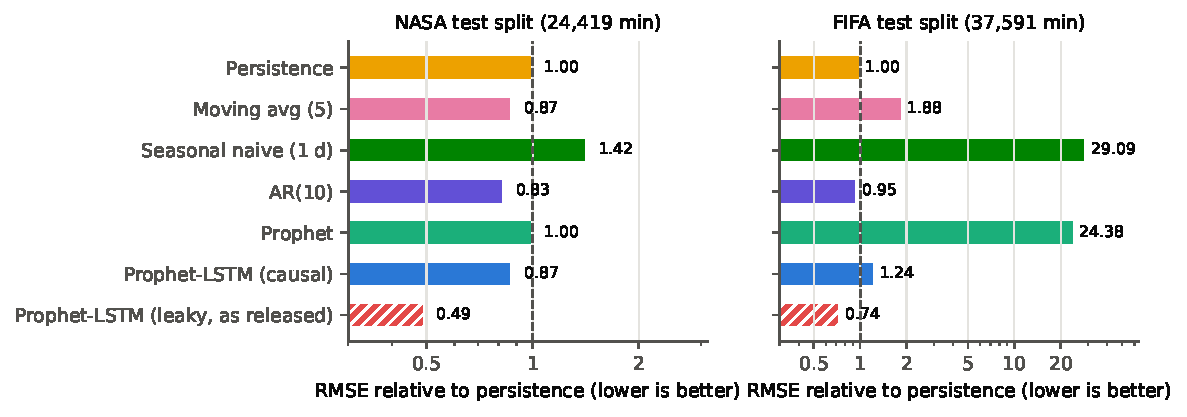
\includegraphics[width=0.85\textwidth]{fig_e1_causal_vs_leaky.pdf}
\caption{One-step-ahead RMSE relative to persistence on the full test splits (log scale). The hatched bar uses
the base paper's mis-aligned evaluation.}\label{fig:e1}
\end{figure*}
\begin{table}[!t]\centering
\caption{E1: $t{+}1$ accuracy in raw requests/minute (NASA 24{,}419 and FIFA 37{,}591 test minutes).}\label{tab:e1}
\small
\fitwidth{\begin{tabular}{lrrrrrr}
\toprule
Forecaster & \multicolumn{3}{c}{NASA} & \multicolumn{3}{c}{FIFA} \\
 & RMSE & MAE & $R^2$ & RMSE & MAE & $R^2$ \\
\midrule
Persistence & 16.40 & 12.28 & 0.579 & 763 & 374 & 0.998 \\
Moving avg (5) & 14.32 & 10.81 & 0.679 & 1431 & 454 & 0.994 \\
Seasonal naive (1 d) & 23.35 & 17.46 & 0.147 & 22190 & 6809 & -0.394 \\
AR(10) & 13.58 & 10.32 & 0.711 & 728 & 375 & 0.998 \\
Prophet & 16.37 & 12.56 & 0.581 & 18599 & 9058 & 0.021 \\
Prophet-LSTM (causal) & 14.32 & 10.94 & 0.679 & 944 & 510 & 0.997 \\
Prophet-LSTM (leaky, as released) & 8.10 & 6.28 & 0.897 & 564 & 310 & 0.999 \\
\bottomrule
\end{tabular}
}
\end{table}

\paragraph{Leakage inflates accuracy by 40--43\,\%.} The leaky evaluation, which writes the forecast for $t{+}1$
into row $t$, under-states the hybrid's RMSE: 8.10 instead of 14.32 on NASA ($-43$\,\%; $R^2$ 0.897 vs.\ 0.679)
and 564 instead of 944 on FIFA ($-40$\,\%). The leaky residual ``forecast'' correlates at 0.9997 (NASA) and 0.9996
(FIFA) with the residual of the \emph{same} row, i.e.\ it is a copy of the value being predicted.

\paragraph{Causal ranking.} On NASA the causal hybrid beats Prophet and persistence (RMSE $-13$\,\%), ties a
5-minute moving average (14.32 vs.\ 14.32) and is beaten by AR(10) (13.58). On FIFA it is 24\,\% \emph{worse}
than persistence (944 vs.\ 763). Prophet alone explains almost none of the FIFA variance ($R^2=0.02$), because the
flat-growth seasonal model cannot represent match-driven flash crowds. AR(10) is again the most accurate (728).
The hybrid's published accuracy advantage is therefore an artefact of the evaluation.

\subsection{E2: Controller cost under CPU budgets (RQ2)}
\begin{figure*}[!t]\centering
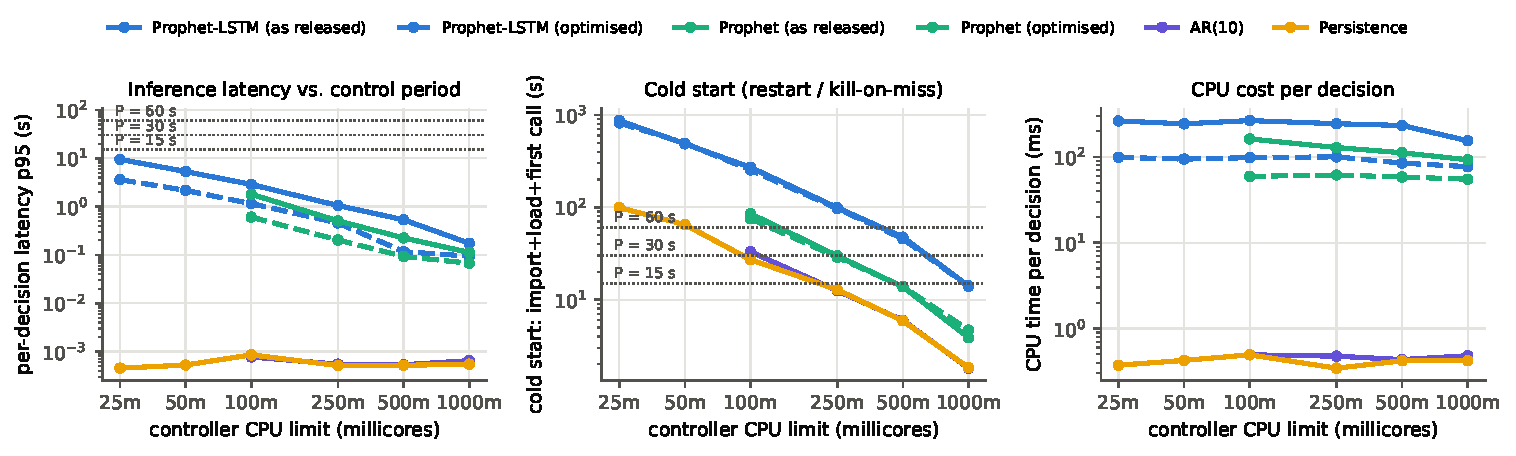
\includegraphics[width=0.85\textwidth]{fig_e2_overhead.pdf}
\caption{E2: p95 per-decision latency, cold start and CPU per decision as a function of the scaler's CPU limit
(FIFA models, log scales). Dotted lines: control periods of 15/30/60\,s. The full per-configuration table
(CPU, latency, throttling, memory) is \texttt{cutoff3/results/e2\_overhead.json} in the repository.}\label{fig:e2}
\end{figure*}
\paragraph{Per-decision inference fits every budget.} Even at 100m, the as-released hybrid needs 266\,ms of CPU
and 2.65\,s of wall time per decision (p95 2.86\,s), less than 20\,\% of a 15\,s period. At 50m the p95 is
5.3\,s, and even at 25m (a fortieth of a core) it is 9.5\,s, still below the 15\,s period. No forecaster misses a
deadline equal to the control period ($P\in\{15,30,60\}$\,s) at any budget.

\paragraph{Throttling inflates CPU cost.} Under tight quotas the same forecast costs more CPU (hybrid: 157\,ms
unlimited vs.\ 266\,ms at 100m), and 100\,\% of CFS periods are throttled at 100m. TensorFlow and Stan create
thread pools sized to the host's cores, and those threads contend inside a 10\,\% quota.

\paragraph{The binding costs are cold start, memory and re-fitting.}
\begin{itemize}
\item \textbf{Cold start.} Import, model load and first call take 270\,s at 100m (18 control periods of 15\,s),
      99\,s at 250m and 48\,s at 500m, rising to 487\,s at 50m and 868\,s at 25m, against 27--33\,s for persistence and AR(10). A kill-and-restart policy is
      therefore dangerous below 500m: one deadline miss leaves the controller on the fallback for minutes.
\item \textbf{Memory.} The hybrid's resident set is $\approx$\,700\,MB, against 170\,MB for Prophet and 90\,MB for
      the light models, independent of the CPU limit.
\item \textbf{Re-fitting} (7-day window, FIFA). Re-fitting Prophet on 7 days takes 64\,s at 100m and one LSTM
      epoch takes 136\,s. A full re-training (6--16 epochs in E1) would take 14--36\,min of controller time, so
      periodic re-training cannot share the controller's budget.
\end{itemize}

\paragraph{Implementation dominates model cost.} Removing Prophet's uncertainty sampling, which the point
forecast does not use, and calling the LSTM directly reduces the hybrid's CPU per decision by 50--64\,\% (266 to
98\,ms at 100m) with identical forecasts.

\subsection{E5a: Deadline sensitivity (RQ2)}
Because no forecast was late at $D=P$, we asked at which deadline the budget starts to bind
(Figure~\ref{fig:deadline}). At 100m, the as-released hybrid misses \emph{every}
deadline of 2\,s or less, and the optimised hybrid misses 40\,\% at $D=1$\,s. At 250m, the released hybrid
misses 17\,\% at 1\,s; at 500m and above, deadlines of 1\,s are met. Below 100m the miss region widens: at 50m
the released hybrid misses every deadline up to 3\,s, and at 25m every deadline up to 5\,s. AR(10) and persistence answer in under 1\,ms
at every budget. A deployment that needs sub-period decisions (for example a 1--2\,s deadline to leave time for
actuation, or a controller that serves many workloads sequentially) therefore needs at least 250--500m per
hybrid forecaster, whereas the lightweight forecasters fit in any budget.

\begin{figure*}[!t]\centering
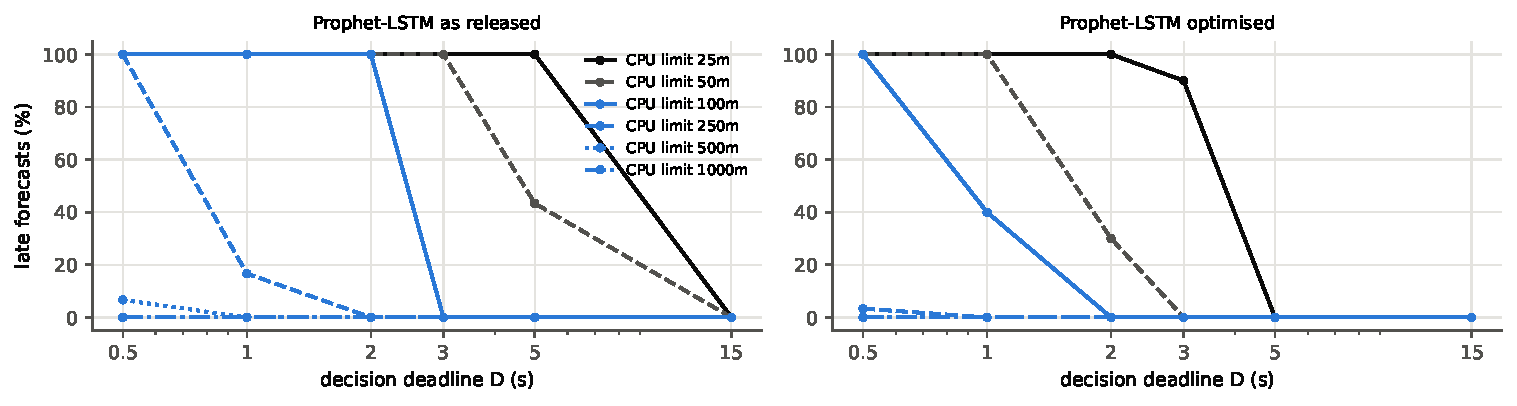
\includegraphics[width=0.85\textwidth]{fig_e5_deadline.pdf}
\caption{E5a: share of late forecasts as a function of the decision deadline $D$, per CPU limit (30 measured
decisions per configuration).}\label{fig:deadline}
\end{figure*}
\subsection{E3: Trace-driven scaling comparison (RQ1, RQ3)}
\begin{figure*}[!t]\centering
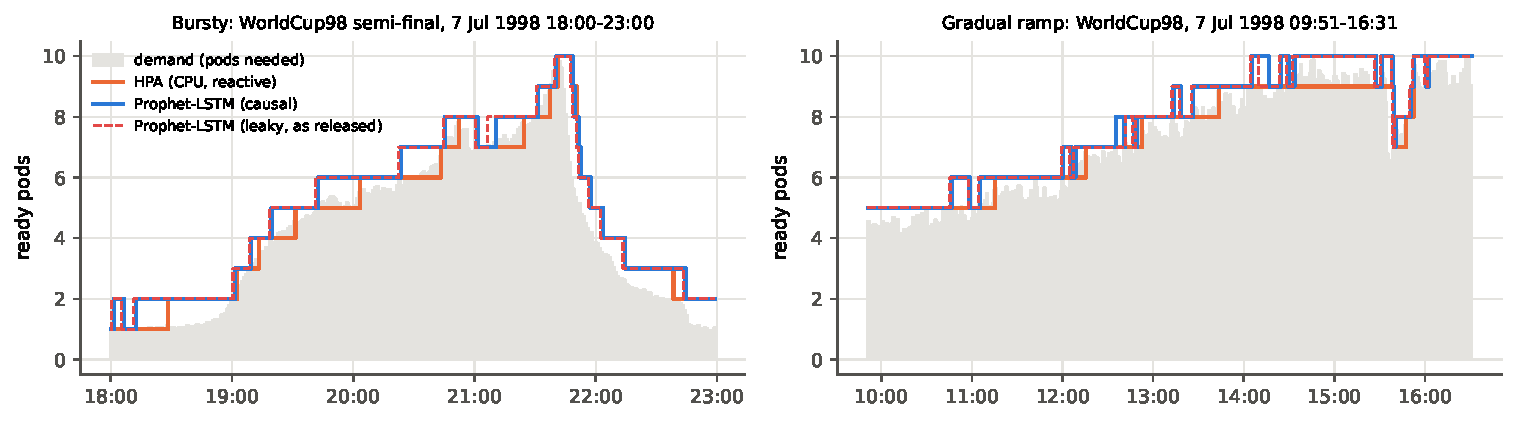
\includegraphics[width=0.85\textwidth]{fig_e3_sim_timeseries.pdf}
\caption{E3: ready pods under the shared replica policy for HPA, the causal hybrid and the leaky hybrid
(\texttt{bursty} and \texttt{ramp}). Grey: pods needed by the demand at the 70\,\% target.}\label{fig:e3ts}
\end{figure*}
\begin{table*}[!t]\centering
\caption{E3: provisioning metrics (start-up delay 0). sat.: share of minutes in which demand exceeded the pods'
full capacity $NC$.}\label{tab:e3}
\scriptsize
\begin{tabular}{llrrrrrr}
\toprule
Scenario & Signal & $\Theta_U$ (\%) & $\Theta_O$ (\%) & $T_U$ (\%) & $T_O$ (\%) & mean pods & sat. (\%) \\
\midrule
steady & HPA (CPU, reactive) & 2.31 & 157.4 & 12.6 & 87.4 & 4.14 & 2.4 \\
 & Persistence & 1.92 & 164.5 & 10.7 & 89.3 & 4.29 & 1.8 \\
 & AR(10) & 3.23 & 129.8 & 17.6 & 82.4 & 3.61 & 3.6 \\
 & Prophet & 2.37 & 150.1 & 13.8 & 86.2 & 3.89 & 1.7 \\
 & Prophet-LSTM (causal) & 1.35 & 167.9 & 9.2 & 90.8 & 4.18 & 0.6 \\
 & Prophet-LSTM (leaky, as released) & 0.44 & 161.9 & 5.7 & 94.3 & 4.18 & 0.1 \\
 & Oracle & 0.00 & 153.7 & 0.0 & 99.9 & 4.29 & 0.0 \\
ramp & HPA (CPU, reactive) & 0.84 & 6.9 & 22.7 & 77.1 & 7.44 & 0.0 \\
 & Persistence & 0.10 & 11.2 & 3.7 & 96.0 & 7.81 & 0.0 \\
 & AR(10) & 0.11 & 11.1 & 4.2 & 95.5 & 7.81 & 0.0 \\
 & Prophet & 4.84 & 25.6 & 44.1 & 55.9 & 9.02 & 0.0 \\
 & Prophet-LSTM (causal) & 0.13 & 11.4 & 4.5 & 95.3 & 7.82 & 0.0 \\
 & Prophet-LSTM (leaky, as released) & 0.01 & 11.1 & 1.2 & 98.5 & 7.80 & 0.0 \\
 & Oracle & 0.00 & 11.3 & 0.0 & 99.8 & 7.83 & 0.0 \\
bursty & HPA (CPU, reactive) & 1.43 & 21.0 & 30.3 & 69.7 & 4.53 & 0.0 \\
 & Persistence & 0.09 & 31.1 & 3.7 & 96.0 & 4.85 & 0.0 \\
 & AR(10) & 0.09 & 31.3 & 3.3 & 96.3 & 4.87 & 0.0 \\
 & Prophet & 58.45 & 0.3 & 92.3 & 7.7 & 1.06 & 77.0 \\
 & Prophet-LSTM (causal) & 0.12 & 33.0 & 3.3 & 96.3 & 4.90 & 0.0 \\
 & Prophet-LSTM (leaky, as released) & 0.02 & 33.2 & 0.7 & 99.0 & 4.92 & 0.0 \\
 & Oracle & 0.00 & 31.2 & 0.0 & 99.7 & 4.86 & 0.0 \\
diurnal & HPA (CPU, reactive) & 1.84 & 102.7 & 11.8 & 87.3 & 4.30 & 1.1 \\
 & Persistence & 1.53 & 108.7 & 10.2 & 89.1 & 4.44 & 0.9 \\
 & AR(10) & 2.74 & 81.9 & 17.9 & 80.3 & 3.79 & 1.7 \\
 & Prophet & 4.82 & 62.2 & 26.5 & 71.2 & 3.46 & 4.8 \\
 & Prophet-LSTM (causal) & 1.89 & 93.0 & 12.8 & 85.7 & 4.04 & 1.2 \\
 & Prophet-LSTM (leaky, as released) & 0.77 & 88.3 & 9.7 & 88.7 & 4.04 & 0.0 \\
 & Oracle & 0.00 & 102.1 & 0.0 & 98.8 & 4.44 & 0.0 \\
\bottomrule
\end{tabular}

\end{table*}
\begin{table*}[!t]\centering
\caption{E5b: paired difference in $\Theta_U$ (percentage points) with 95\,\% moving-block bootstrap confidence
intervals (block 30\,min, 2000 resamples). Negative values favour the row's scaler. Last column: share of minutes
in which the scaler provisions exactly as many pods as the persistence scaler.}\label{tab:boot}
\scriptsize
\fitwidth{\begin{tabular}{@{}llrrr@{}}\toprule
Scenario & Scaler & $\Delta\Theta_U$ vs.\ HPA (pp) & $\Delta\Theta_U$ vs.\ persistence (pp) & same pods as pers.\ (\%) \\ \midrule
steady & AR(10) & +0.92 [+0.66, +1.20] & +1.31 [+1.04, +1.62] & 40.3 \\
 & Prophet (B2) & +0.06 [-0.60, +0.84] & +0.45 [-0.24, +1.25] & 35.1 \\
 & Prophet--LSTM & -0.96 [-1.26, -0.69] & -0.57 [-0.84, -0.31] & 55.7 \\
 & Persistence & -0.39 [-0.58, -0.25] & --- & 100.0 \\
\midrule
diurnal & AR(10) & +0.89 [+0.58, +1.21] & +1.20 [+0.88, +1.54] & 40.5 \\
 & Prophet (B2) & +2.98 [+2.00, +4.17] & +3.29 [+2.34, +4.44] & 26.5 \\
 & Prophet--LSTM & +0.05 [-0.16, +0.27] & +0.36 [+0.16, +0.57] & 53.8 \\
 & Persistence & -0.31 [-0.43, -0.20] & --- & 100.0 \\
\midrule
ramp & AR(10) & -0.73 [-1.19, -0.41] & +0.01 [+0.00, +0.04] & 96.0 \\
 & Prophet (B2) & +4.00 [+0.93, +7.70] & +4.74 [+1.84, +8.31] & 15.7 \\
 & Prophet--LSTM & -0.71 [-1.17, -0.39] & +0.03 [-0.01, +0.09] & 94.3 \\
 & Persistence & -0.75 [-1.21, -0.42] & --- & 100.0 \\
\midrule
bursty & AR(10) & -1.34 [-2.15, -0.79] & -0.00 [-0.01, +0.00] & 97.3 \\
 & Prophet (B2) & +57.02 [+44.00, +76.09] & +58.36 [+45.25, +77.89] & 2.7 \\
 & Prophet--LSTM & -1.31 [-2.07, -0.77] & +0.03 [-0.04, +0.14] & 91.0 \\
 & Persistence & -1.34 [-2.15, -0.79] & --- & 100.0 \\
\bottomrule\end{tabular}
}
\end{table*}

\paragraph{Request-rate scaling beats the CPU HPA on non-stationary load.} On \texttt{ramp} and \texttt{bursty},
persistence, AR(10) and the causal hybrid all reduce $\Theta_U$ from 0.84--1.43\,\% (HPA) to about 0.1\,\%, and
the time under-provisioned from 23--30\,\% to 3--4.5\,\%, for 5--8\,\% more pod-minutes. All three differences to
the HPA are significant (Table~\ref{tab:boot}; e.g.\ \texttt{bursty}: hybrid $-1.31$\,pp [$-2.07$, $-0.77$]).

\paragraph{But the forecaster adds nothing on those scenarios.} The difference between the hybrid and persistence
is $+0.03$\,pp on both \texttt{ramp} [$-0.01$, $+0.09$] and \texttt{bursty} [$-0.04$, $+0.14$]: not significant,
and pointing in the persistence's favour. The hybrid requests exactly the same number of pods as persistence in
94\,\% (\texttt{ramp}) and 91\,\% (\texttt{bursty}) of minutes, and its forecast correlates at 0.999 with the last
observed value. On these workloads the gain over the HPA comes from the \emph{signal}, a request rate with no CPU
saturation and no tolerance band, not from forecasting.

\paragraph{The hybrid helps only on smooth, low, seasonal load.} On NASA \texttt{steady} the hybrid is the only
causal scaler that significantly beats persistence ($-0.57$\,pp [$-0.84$, $-0.31$]; $\Theta_U$ 1.35\,\% vs.\
1.92\,\%), for 3\,\% fewer pod-minutes. On \texttt{diurnal} it is significantly \emph{worse} than persistence
($+0.36$\,pp [$+0.16$, $+0.57$]) and indistinguishable from the HPA. The absolute differences are below 1
percentage point in all NASA cases.

\paragraph{Prophet alone is unsafe on bursty load.} Prophet's seasonal forecast misses the semi-final flash crowd
entirely: demand exceeds full capacity in 77\,\% of minutes and $\Theta_U=58$\,\% (+57\,pp vs.\ HPA,
[+44, +76]). This is the failure mode that the residual LSTM corrects, and it is why the hybrid behaves like a
last-value predictor on FIFA.

\paragraph{Leakage also inflates scaling quality.} Driven by the leaky series, the hybrid looks 3--13$\times$
better than its causal version ($\Theta_U$ 0.02 vs.\ 0.12 on \texttt{bursty}; 0.44 vs.\ 1.35 on
\texttt{steady}), so an offline autoscaling evaluation built on the leaky forecasts would overstate the benefit
too. With a one-step pod start-up delay all scalers degrade slightly and the ranking is unchanged.

\subsection{E4: Live Kubernetes comparison (RQ2, RQ3)}
\begin{figure}[!t]\centering
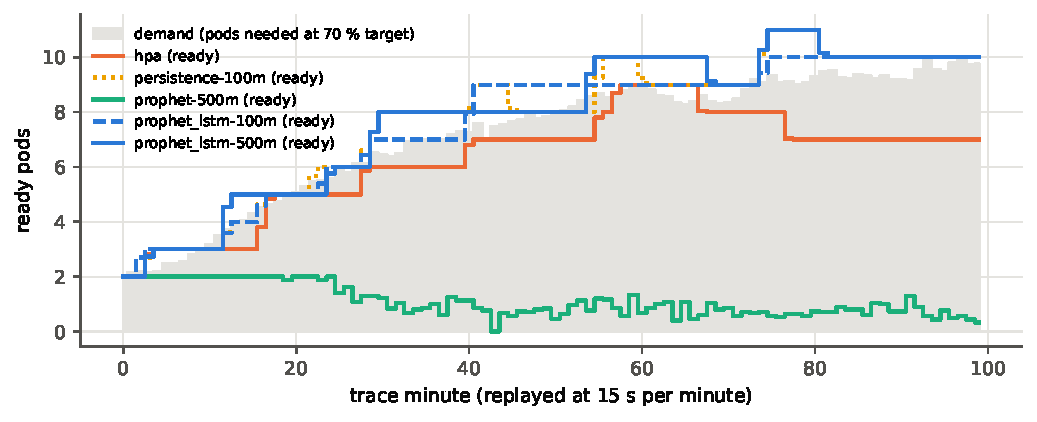
\includegraphics[width=\columnwidth]{fig_e4_live.pdf}
\caption{E4: ready \texttt{work} pods during the live replay of the \texttt{bursty} slice on kind (seed 1).
Grey: pods needed by the offered load at the 70\,\% target.}\label{fig:e4}
\end{figure}
\begin{table*}[!t]\centering
\caption{E4 repetitions: mean $\pm$ standard deviation over load-generator seeds. Ready after: time until the
scaler's first forecast was available (cold start inside the cluster).}\label{tab:e4reps}
\scriptsize
\fitwidth{\begin{tabular}{@{}lcllllll@{}}\toprule
Autoscaler & $n$ & $\Theta_U$ (\%) & $T_U$ (\%) & Pod-min & SLO viol.\ (\%) & Late (\%) & Ready after (s) \\ \midrule
B1: HPA (CPU 70\,\%) & 3 & 21.10 $\pm$ 7.93 & 91.0 $\pm$ 10.6 & 563 $\pm$ 57 & 0.74 $\pm$ 0.32 & --- & --- \\
B2: Prophet @500m & 2 & 77.58 $\pm$ 0.63 & 99.0 $\pm$ 0.0 & 107 $\pm$ 5 & 90.76 $\pm$ 1.11 & 0.0 $\pm$ 0.0 & 22 $\pm$ 3 \\
Persistence @100m & 3 & 0.78 $\pm$ 0.02 & 20.7 $\pm$ 1.5 & 759 $\pm$ 4 & 0.17 $\pm$ 0.14 & 0.0 $\pm$ 0.0 & 86 $\pm$ 3 \\
Prophet--LSTM @100m & 3 & 0.93 $\pm$ 0.45 & 19.0 $\pm$ 4.4 & 764 $\pm$ 4 & 0.47 $\pm$ 0.13 & 0.0 $\pm$ 0.0 & 356 $\pm$ 25 \\
Prophet--LSTM @500m & 3 & 0.66 $\pm$ 0.13 & 15.0 $\pm$ 1.0 & 776 $\pm$ 10 & 0.27 $\pm$ 0.19 & 0.0 $\pm$ 0.0 & 56 $\pm$ 7 \\
\bottomrule\end{tabular}
}
\end{table*}
%E4REPS-BEGIN
\paragraph{The budgeted hybrid works inside a live controller, even at 100m.} Across all six hybrid runs
(three seeds at 100m and three at 500m) not a single forecast was late, and the scaler stayed within its CPU limit
(230\,ms CPU and 2.7\,s p95 latency per decision at 100m, 194\,ms and 0.42\,s at 500m). The cost that
the repetitions make visible is again cold start: inside the cluster the 100m scaler needed
$356\pm25$\,s before its first forecast, against $56\pm7$\,s at 500m and $86\pm3$\,s for persistence at 100m
(Table~\ref{tab:e4reps}). During that time the scaler serves the persistence fallback.

\paragraph{Every request-rate scaler beats the HPA in every seed.} The HPA's under-provisioning varies strongly
with the load pattern ($\Theta_U$ 12.1, 27.1 and 24.0\,\% for seeds 1--3; mean $21.1\pm7.9$\,\%), because its CPU
signal saturates and it scales down inside the tolerance band while demand is still high. Persistence and the
hybrid reduce $\Theta_U$ to below 1.5\,\% in every run (paired differences against the HPA: $-11$ to $-27$\,pp),
at the cost of 35--40\,\% more pod-minutes, i.e.\ the capacity the HPA failed to provision. Request-level SLO
violations stay below 1\,\% for all four of these scalers.

\paragraph{The hybrid does not beat persistence live either.} Persistence is the most stable scaler
($\Theta_U=0.78\pm0.02$\,\%). The hybrid at 100m is on average slightly worse ($0.93\pm0.45$\,\%; paired
differences $-0.12$, $-0.08$ and $+0.66$\,pp), and the hybrid at 500m slightly better ($0.66\pm0.13$\,\%; paired
$-0.03$ to $-0.24$\,pp) while using 1--3\,\% more pod-minutes. In all six paired runs the hybrid had slightly
\emph{more} SLO violations than persistence ($+0.04$ to $+0.53$\,pp), and its live $t{+}1$ RMSE equals that of
persistence (2.28 vs.\ 2.29 req/s at 100m; 2.16 vs.\ 2.17 at 500m). These differences are a fraction of a
percentage point, within seed-to-seed variation, and consistent with the simulator's bootstrap result that the
hybrid and persistence are indistinguishable on \texttt{bursty}. The 0.54 vs.\ 0.06\,\% SLO gap between the
seed-1 hybrid runs at 100m and 500m does not persist across seeds ($0.47\pm0.13$ vs.\ $0.27\pm0.19$\,\%), so we
do not attribute it to the budget.

\paragraph{Prophet alone fails again.} The repeated Prophet@500m run reproduces the collapse: $\Theta_U=78$\,\%,
92\,\% of requests violate the SLO, and the forecast never anticipates the flash crowd.
%E4REPS-END

%=====================================================================
\section{Discussion}\label{sec:discussion}
\paragraph{RQ1: validity.} The base paper's accuracy claim does not survive a causal evaluation. The leaky
protocol makes the hybrid look 40--43\,\% more accurate and 3--13$\times$ better at provisioning than it is. Under
the causal protocol, a least-squares AR(10) model, which costs half a millisecond, is the most accurate
forecaster on both traces. This is the pattern that Kapoor and Narayanan~\cite{kapoor2023} describe for leakage in
general: when the leak is removed, the complex model's advantage over the simple one disappears. It also agrees
with the M-competition evidence that simple statistical methods are hard to beat~\cite{makridakis2018}.

\paragraph{RQ2: cost.} The hybrid \emph{can} run inside a controller budget, which answers the feasibility part
of our question positively: at 100m it uses about a third of the scaler's quota and never misses a 15\,s
deadline, live (six runs, three seeds) or offline, and offline even 25m meets the 15\,s period. But the cost is concentrated where accuracy tables do not look. Cold start is 18--24
control periods at 100m (270\,s offline, $356\pm25$\,s live), memory is 4--8 times that of the lightweight forecasters, re-training cannot be done
inside the budget, and sub-2\,s deadlines are missed at 100m. The budget therefore constrains \emph{operations}
(restarts, controller scale-out, model refresh, multi-tenant controllers) rather than steady-state inference.
A practical consequence is that kill-on-miss, a natural way to enforce a deadline, is harmful below 500m: it turns
one slow forecast into minutes without forecasts.

\paragraph{RQ3: benefit.} Request-rate scaling is clearly better than CPU-based HPA on non-stationary load, both
simulated and live. The HPA's CPU signal saturates at the pod limit and moves inside the 10\,\% tolerance band, so
it lags ramps and even scales down while demand stays high (Fig.~\ref{fig:e4}). However, a persistence
forecaster in the same policy captures this gain. Over three live seeds, the hybrid's $\Theta_U$ differs from persistence by less than 0.7\,pp in either direction,
its live forecast has the same RMSE as persistence, and
in simulation it provisions the same pods as persistence in more than 90\,\% of FIFA minutes. Its only significant
advantage appears on smooth, low NASA load, and it is below one percentage point of $\Theta_U$. Prophet alone, the
B2 baseline, is unsafe on flash crowds.

\paragraph{When does the hybrid pay off?} Our evidence suggests three conditions together: (i)~strong, stable
seasonality that a last-value predictor cannot anticipate; (ii)~a control period or pod start-up long enough that
anticipating the next period matters; and (iii)~enough controller budget ($\geq$500m and $\approx$1\,GB) to absorb
cold start and re-training. On the bursty, match-driven WorldCup98 load none of these hold, and on NASA only the
first does. For most Kubernetes services, scaling on the request rate with a persistence or AR forecaster gives
the benefit at negligible cost.

\paragraph{Implications.} For practitioners: switch the HPA to a request-rate metric before adding a forecaster,
and budget the forecaster's cold start and memory, not only its inference time. For researchers: evaluate
autoscaling forecasters causally, include a persistence forecaster under the same replica policy as a mandatory
control, and report controller-side cost on stated hardware and budgets.

%=====================================================================
\section{Limitations and Future Work}\label{sec:limits}
\emph{Internal validity:} the live cluster shares one host with its load generator; runs were sequential and E4
was repeated with three seeds, but host noise remains, and E2 uses 30 decisions per configuration.
\emph{Time compression:} one trace minute is replayed in 15\,s, so pod start-up (2--3\,s) is relatively slower
than in real time, which favours anticipation; our finding that forecasting adds little is thus conservative.
\emph{External validity:} two 1990s traces, one synthetic CPU-bound service, one horizon ($t{+}1$) and one hybrid
model; modern microservices, multi-step horizons and other deep forecasters may behave differently.
\emph{Construct validity:} only the scaler Pod is budgeted, and the 500\,ms SLO and 70\,\% target are single
choices. \emph{Conclusion validity:} three live repetitions give limited power, so significance rests on the
simulator's bootstrap intervals and the live runs confirm direction and feasibility.

Future work should study multi-step horizons and longer pod start-up, where anticipation matters more; other
forecaster families and online model selection under the same budget~\cite{toka2021}; re-training in a separate
scheduled Job and the effect of model staleness; multi-node clusters, microservice benchmarks and modern traces;
and a deadline policy safer than kill-on-miss, such as cancelling one request without restarting the worker.

%=====================================================================
\section{Conclusion}\label{sec:conclusion}
We evaluated a published Prophet--LSTM predictive autoscaler causally and inside a CPU-limited Kubernetes
controller. The hybrid fits the budget for steady-state inference, even at a tenth of a core, but its published
accuracy advantage is produced by a non-causal evaluation. Its real costs are cold start, memory and re-training.
Its scaling benefit over the HPA is matched by a persistence forecaster under the same replica policy. The answer
to our research question is therefore: \emph{yes, it fits, but it does not pay}. On the evaluated workloads, the
improvement attributed to forecasting is an improvement from scaling on the request rate. Causal evaluation, a
persistence control and controller-side cost measurement should become standard in autoscaling research.

\section*{Acknowledgements}
We thank our supervisor, Basharat Hussain, for guidance. We thank P.\,B.\ Guruge and Y.\,H.\,P.\,P.\
Priyadarshana for releasing their code, models and data, without which this study would not have been possible.

\section*{Use of AI tools}
AI assistants were used for debugging help, language editing and code review. All experiments were executed by
the authors on the stated hardware; all numbers come from the released result files, and all references were
checked against their sources.

\section*{Data and code availability}
Code, trained models, raw results, figure scripts and reproduction instructions:
\url{https://github.com/Saadx-git/Cloud_project_I230822_I230651}. The NASA-HTTP and WorldCup98 traces are
publicly available from the Internet Traffic Archive; the per-minute series are taken from the base paper's
repository (CC BY 4.0).

%=====================================================================
\begin{thebibliography}{99}\footnotesize
% All references are journal articles; every DOI was verified against Crossref (Nov 2026).
\bibitem{burns2016} B.\ Burns, B.\ Grant, D.\ Oppenheimer, E.\ Brewer and J.\ Wilkes, ``Borg, Omega, and Kubernetes,'' \textit{Communications of the ACM}, vol.~59, no.~5, pp.~50--57, 2016, doi:10.1145/2890784.
\bibitem{nguyen2020} T.-T.\ Nguyen, Y.-J.\ Yeom, T.\ Kim, D.-H.\ Park and S.\ Kim, ``Horizontal pod autoscaling in Kubernetes for elastic container orchestration,'' \textit{Sensors}, vol.~20, no.~16, Art.~4621, 2020, doi:10.3390/s20164621.
\bibitem{lorido2014} T.\ Lorido-Botran, J.\ Miguel-Alonso and J.\,A.\ Lozano, ``A review of auto-scaling techniques for elastic applications in cloud environments,'' \textit{Journal of Grid Computing}, vol.~12, no.~4, pp.~559--592, 2014, doi:10.1007/s10723-014-9314-7.
\bibitem{qu2018} C.\ Qu, R.\,N.\ Calheiros and R.\ Buyya, ``Auto-scaling web applications in clouds: A taxonomy and survey,'' \textit{ACM Computing Surveys}, vol.~51, no.~4, Art.~73, 2018, doi:10.1145/3148149.
\bibitem{aldhuraibi2018} Y.\ Al-Dhuraibi, F.\ Paraiso, N.\ Djarallah and P.\ Merle, ``Elasticity in cloud computing: State of the art and research challenges,'' \textit{IEEE Transactions on Services Computing}, vol.~11, no.~2, pp.~430--447, 2018, doi:10.1109/TSC.2017.2711009.
\bibitem{dogani2023} J.\ Dogani, R.\ Namvar and F.\ Khunjush, ``Auto-scaling techniques in container-based cloud and edge/fog computing: Taxonomy and survey,'' \textit{Computer Communications}, vol.~209, pp.~120--150, 2023, doi:10.1016/j.comcom.2023.06.010.
\bibitem{calheiros2015} R.\,N.\ Calheiros, E.\ Masoumi, R.\ Ranjan and R.\ Buyya, ``Workload prediction using ARIMA model and its impact on cloud applications' QoS,'' \textit{IEEE Transactions on Cloud Computing}, vol.~3, no.~4, pp.~449--458, 2015, doi:10.1109/TCC.2014.2350475.
\bibitem{imdoukh2020} M.\ Imdoukh, I.\ Ahmad and M.\,G.\ Alfailakawi, ``Machine learning-based auto-scaling for containerized applications,'' \textit{Neural Computing and Applications}, vol.~32, no.~13, pp.~9745--9760, 2020, doi:10.1007/s00521-019-04507-z.
\bibitem{dangquang2021} N.-M.\ Dang-Quang and M.\ Yoo, ``Deep learning-based autoscaling using bidirectional long short-term memory for Kubernetes,'' \textit{Applied Sciences}, vol.~11, no.~9, Art.~3835, 2021, doi:10.3390/app11093835.
\bibitem{guruge2025} P.\,B.\ Guruge and Y.\,H.\,P.\,P.\ Priyadarshana, ``Time series forecasting-based Kubernetes autoscaling using Facebook Prophet and Long Short-Term Memory,'' \textit{Frontiers in Computer Science}, vol.~7, Art.~1509165, 2025, doi:10.3389/fcomp.2025.1509165.
\bibitem{taylor2018} S.\,J.\ Taylor and B.\ Letham, ``Forecasting at scale,'' \textit{The American Statistician}, vol.~72, no.~1, pp.~37--45, 2018, doi:10.1080/00031305.2017.1380080.
\bibitem{hochreiter1997} S.\ Hochreiter and J.\ Schmidhuber, ``Long short-term memory,'' \textit{Neural Computation}, vol.~9, no.~8, pp.~1735--1780, 1997, doi:10.1162/neco.1997.9.8.1735.
\bibitem{gari2021} Y.\ Gar\'i, D.\,A.\ Monge, E.\ Pacini, C.\ Mateos and C.\ Garc\'ia Garino, ``Reinforcement learning-based application autoscaling in the cloud: A survey,'' \textit{Engineering Applications of Artificial Intelligence}, vol.~102, Art.~104288, 2021, doi:10.1016/j.engappai.2021.104288.
\bibitem{zhong2022} Z.\ Zhong, M.\ Xu, M.\,A.\ Rodriguez, C.\ Xu and R.\ Buyya, ``Machine learning-based orchestration of containers: A taxonomy and future directions,'' \textit{ACM Computing Surveys}, vol.~54, no.~10s, pp.~1--35, 2022, doi:10.1145/3510415.
\bibitem{gandhi2012} A.\ Gandhi, M.\ Harchol-Balter, R.\ Raghunathan and M.\,A.\ Kozuch, ``AutoScale: Dynamic, robust capacity management for multi-tier data centers,'' \textit{ACM Transactions on Computer Systems}, vol.~30, no.~4, pp.~1--26, 2012, doi:10.1145/2382553.2382556.
\bibitem{kumar2018} J.\ Kumar and A.\,K.\ Singh, ``Workload prediction in cloud using artificial neural network and adaptive differential evolution,'' \textit{Future Generation Computer Systems}, vol.~81, pp.~41--52, 2018, doi:10.1016/j.future.2017.10.047.
\bibitem{joshi2024} N.\,S.\ Joshi, R.\ Raghuwanshi, Y.\,M.\ Agarwal, B.\ Annappa and D.\,N.\ Sachin, ``ARIMA-PID: container auto scaling based on predictive analysis and control theory,'' \textit{Multimedia Tools and Applications}, vol.~83, no.~9, pp.~26369--26386, 2024, doi:10.1007/s11042-023-16587-0.
\bibitem{lanciano2024} G.\ Lanciano, F.\ Galli, T.\ Cucinotta, D.\ Bacciu and A.\ Passarella, ``Extending OpenStack Monasca for predictive elasticity control,'' \textit{Big Data Mining and Analytics}, vol.~7, no.~2, pp.~315--339, 2024, doi:10.26599/BDMA.2023.9020014.
\bibitem{amiri2017} M.\ Amiri and L.\ Mohammad-Khanli, ``Survey on prediction models of applications for resources provisioning in cloud,'' \textit{Journal of Network and Computer Applications}, vol.~82, pp.~93--113, 2017, doi:10.1016/j.jnca.2017.01.016.
\bibitem{masdari2020} M.\ Masdari and A.\ Khoshnevis, ``A survey and classification of the workload forecasting methods in cloud computing,'' \textit{Cluster Computing}, vol.~23, no.~4, pp.~2399--2424, 2020, doi:10.1007/s10586-019-03010-3.
\bibitem{bauer2020} A.\ Bauer, M.\ Z\"ufle, N.\ Herbst, A.\ Zehe, A.\ Hotho and S.\ Kounev, ``Time series forecasting for self-aware systems,'' \textit{Proceedings of the IEEE}, vol.~108, no.~7, pp.~1068--1093, 2020, doi:10.1109/JPROC.2020.2983857.
\bibitem{bauer2019} A.\ Bauer, N.\ Herbst, S.\ Spinner, A.\ Ali-Eldin and S.\ Kounev, ``Chameleon: A hybrid, proactive auto-scaling mechanism on a level-playing field,'' \textit{IEEE Transactions on Parallel and Distributed Systems}, vol.~30, no.~4, pp.~800--813, 2019, doi:10.1109/TPDS.2018.2870389.
\bibitem{toka2021} L.\ Toka, G.\ Dobreff, B.\ Fodor and B.\ Sonkoly, ``Machine learning-based scaling management for Kubernetes edge clusters,'' \textit{IEEE Transactions on Network and Service Management}, vol.~18, no.~1, pp.~958--972, 2021, doi:10.1109/TNSM.2021.3052837.
\bibitem{makridakis2020} S.\ Makridakis, E.\ Spiliotis and V.\ Assimakopoulos, ``The M4 Competition: 100,000 time series and 61 forecasting methods,'' \textit{International Journal of Forecasting}, vol.~36, no.~1, pp.~54--74, 2020, doi:10.1016/j.ijforecast.2019.04.014.
\bibitem{hewamalage2021} H.\ Hewamalage, C.\ Bergmeir and K.\ Bandara, ``Recurrent neural networks for time series forecasting: Current status and future directions,'' \textit{International Journal of Forecasting}, vol.~37, no.~1, pp.~388--427, 2021, doi:10.1016/j.ijforecast.2020.06.008.
\bibitem{herbst2018} N.\ Herbst, A.\ Bauer, S.\ Kounev, G.\ Oikonomou, E.\ van Eyk, G.\ Kousiouris, A.\ Evangelinou, R.\ Krebs, T.\ Brecht, C.\,L.\ Abad and A.\ Iosup, ``Quantifying cloud performance and dependability: Taxonomy, metric design, and emerging challenges,'' \textit{ACM Transactions on Modeling and Performance Evaluation of Computing Systems}, vol.~3, no.~4, Art.~19, 2018, doi:10.1145/3236332.
\bibitem{makridakis2018} S.\ Makridakis, E.\ Spiliotis and V.\ Assimakopoulos, ``Statistical and machine learning forecasting methods: Concerns and ways forward,'' \textit{PLoS ONE}, vol.~13, no.~3, Art.~e0194889, 2018, doi:10.1371/journal.pone.0194889.
\bibitem{kapoor2023} S.\ Kapoor and A.\ Narayanan, ``Leakage and the reproducibility crisis in machine-learning-based science,'' \textit{Patterns}, vol.~4, no.~9, Art.~100804, 2023, doi:10.1016/j.patter.2023.100804.
\bibitem{tashman2000} L.\,J.\ Tashman, ``Out-of-sample tests of forecasting accuracy: An analysis and review,'' \textit{International Journal of Forecasting}, vol.~16, no.~4, pp.~437--450, 2000, doi:10.1016/S0169-2070(00)00065-0.
\bibitem{bergmeir2012} C.\ Bergmeir and J.\,M.\ Ben\'itez, ``On the use of cross-validation for time series predictor evaluation,'' \textit{Information Sciences}, vol.~191, pp.~192--213, 2012, doi:10.1016/j.ins.2011.12.028.
\bibitem{hyndman2006} R.\,J.\ Hyndman and A.\,B.\ Koehler, ``Another look at measures of forecast accuracy,'' \textit{International Journal of Forecasting}, vol.~22, no.~4, pp.~679--688, 2006, doi:10.1016/j.ijforecast.2006.03.001.
\bibitem{diebold1995} F.\,X.\ Diebold and R.\,S.\ Mariano, ``Comparing predictive accuracy,'' \textit{Journal of Business \& Economic Statistics}, vol.~13, no.~3, pp.~253--263, 1995, doi:10.1080/07350015.1995.10524599.
\bibitem{arlitt1997} M.\,F.\ Arlitt and C.\,L.\ Williamson, ``Internet Web servers: Workload characterization and performance implications,'' \textit{IEEE/ACM Transactions on Networking}, vol.~5, no.~5, pp.~631--645, 1997, doi:10.1109/90.649565.
\bibitem{arlitt2000} M.\ Arlitt and T.\ Jin, ``A workload characterization study of the 1998 World Cup Web site,'' \textit{IEEE Network}, vol.~14, no.~3, pp.~30--37, 2000, doi:10.1109/65.844498.
\bibitem{kunsch1989} H.\,R.\ K\"unsch, ``The jackknife and the bootstrap for general stationary observations,'' \textit{The Annals of Statistics}, vol.~17, no.~3, pp.~1217--1241, 1989, doi:10.1214/aos/1176347265.
\bibitem{efron1979} B.\ Efron, ``Bootstrap methods: Another look at the jackknife,'' \textit{The Annals of Statistics}, vol.~7, no.~1, pp.~1--26, 1979, doi:10.1214/aos/1176344552.
\bibitem{politis1994} D.\,N.\ Politis and J.\,P.\ Romano, ``The stationary bootstrap,'' \textit{Journal of the American Statistical Association}, vol.~89, no.~428, pp.~1303--1313, 1994, doi:10.1080/01621459.1994.10476870.
\end{thebibliography}

%=====================================================================
\section*{Authors' Profiles}
\paragraph{Saad Azhar} (i230822@isb.nu.edu.pk) is a final-year BS Computer Science student at FAST-NUCES,
Islamabad, interested in cloud computing, container orchestration and machine-learning systems. Saad maintains the
public repository, worked on the reproduction and code audit and on the experimental framework, and co-wrote the
manuscript.

\paragraph{Syed Ali Ramish Abidi} (i230651@isb.nu.edu.pk) is a final-year BS Computer Science student at
FAST-NUCES, Islamabad, interested in distributed systems, Kubernetes and performance evaluation. Ali Ramish built the live
Kubernetes testbed, ran the controller-cost and live experiments, carried out the statistical analysis, and
co-wrote the manuscript.

\end{document}
